\documentclass[12pt,letterpaper]{article}
\usepackage[UTF8]{ctex}
\usepackage{fullpage}
\usepackage[top=2cm, bottom=4.5cm, left=2.5cm, right=2.5cm]{geometry}
\usepackage{amsmath,amsthm,amsfonts,amssymb,amscd}
\usepackage{lastpage}
\usepackage{enumerate}
\usepackage{fancyhdr}
\usepackage{mathrsfs}
\usepackage{xcolor}
\usepackage{graphicx}
\usepackage{listings}
\usepackage{hyperref}
\usepackage{dot2texi}
\usepackage{tikz}
\usepackage{float}
\usepackage[pdf]{graphviz}
\usetikzlibrary{automata,shapes,arrows} 

\hypersetup{%
  colorlinks=true,
  linkcolor=blue,
  linkbordercolor={0 0 1}
}
 
\renewcommand\lstlistingname{Algorithm}
\renewcommand\lstlistlistingname{Algorithms}
\def\lstlistingautorefname{Alg.}

\lstdefinestyle{Matlab}{
    language        = matlab,
    frame           = lines, 
    basicstyle      = \footnotesize,
    keywordstyle    = \color{blue},
    stringstyle     = \color{green},
    commentstyle    = \color{red}\ttfamily
}
\setlength{\parindent}{0.0in}
\setlength{\parskip}{0.05in}

% Edit these as appropriate
\newcommand\course{自然语言处理基础}
\newcommand\hwnumber{2}                  % <-- homework number
\newcommand\name{唐一早}                 % <-- Name
\newcommand\ID{2100012613}           % <-- ID

\pagestyle{fancyplain}
\headheight 35pt
\lhead{\name\\\ID}                 
\chead{\textbf{\Large Homework \hwnumber}}
\rhead{\course \\ \today}
\lfoot{}
\cfoot{}
\rfoot{\small\thepage}
\headsep 1.5em



\title{Lab2 Report}
\begin{document}

\maketitle

\section{Problem 1}

\subsection{Q1}

最中得到的词汇表大小为16050,原训练集的单词数量为107259,经过BPE方法tokenize后得到的token数量为124695。

\subsection{Q2}

通过BPE方法的得到的测试数据的总token数量为2092,其中<unk>字符数量为105,且均非英文字符。
事实上因为BPE方法是从字符开始不断结合bigram来进行tokenization。因此只要是用同一种字符构筑的语言都可以被识别并且被tokenize,只有用tokenizer没见过的字符才会被识别成<unk>。
而普通的按照空格或符号分词的方法一旦遇到未出现过的单词就会被分为<unk>,更不用说未见过的字符和语言。
所以BPE方法得到<unk>的概率一定比按单词分词的方法好。

\section{Problem 2}

\subsection{Method}

\subsubsection{BPE}

如problem1中所实现的,从字母开始,不断找词频最高、且连续的两个token合并,直到达到目标词数。
没有空格的语言也可以分词,没遇见过的word会按出现频率最高的subword,但是遇到没有遇见过的语言会全部识别为unk。

\subsubsection{BBPE}

BBPE核心思想将BPE的从字符级别扩展到子节(Byte)级别。
采用BBPE的好处是可以跨语言共用词表,显著压缩词表的大小。而坏处就是,对于类似中文这样的语言,一段文字的序列长度会显著增长。
因此,BBPE可能比BPE表现的更好。然而,BBPE sequence比起BPE来说略长,这也导致了更长的训练/推理时间。

\subsubsection{WordPiece}

WordPiece算法可以看作是BPE的变种,采用的不是bigram的频率而是两个subtoken之间的互信息作为标准。因此其分词结果会和BPE类似。

\subsubsection{Unigram}

Unigram Language Model 先初始一个大词表,接着通过语言模型评估subword概率不断减少词表,直到限定词汇量。显然因为最终没有显示的tokenize方法,要对单词尝试所有种类的tokenize可能,这种方法在tokenize和训练速度上比较慢。
\subsubsection{SentencePiece}

SentencePiece是把一个句子看作一个整体,再拆成片段,而没有保留天然的词语的概念。一般地,它把空格也当作一种特殊字符来处理,再用BPE或者Unigram算法来构造词汇表。
因而有没有空格对SentencePiece来说没什么分别,所以也可以做中文分词。根据使用算法不同,在unk字符数量和数字tokenize上表现不同。

\begin{figure}[h]
  \centering
  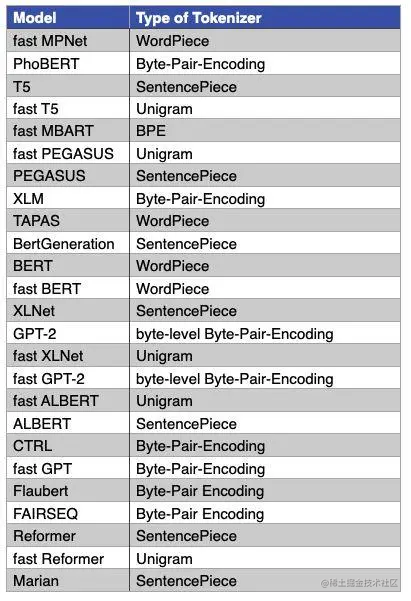
\includegraphics[width=0.5\textwidth]{tokenizers.png}
  \caption{各个语言模型所使用的tokenization方法}
  \label{fig:example}
\end{figure}


\subsection{Examples}
所有案例在test.ipynb中测试,具体案例可以前往查看

\subsubsection{Bert}

Bert使用wordpiece方法,在分词时会按标点和空格先分词,再对单词分词。因而“don't”会被分为“don” “'” “t”。在中文分词上是一个字一个字分,在数字上会把小数拆开,会把较长的数字分为较短的数字。

\subsubsection{gpt}

gpt系列使用的是BBPE方法,在分词时也会按标点和空格先分词,再对单词分词。中文和数字上分词效果和bert类似,区别是gpt1对长数字分词每个小数字的长度比gpt2短一些

\subsubsection{t5 \& XLNet}
t5和XLNet采用的是SentencePiece方法,分词结果类似,在英文分词里偶尔会拆出一些单个字母,分数字情况和以上类似,分中文时会将标点之间的所有中文分为一个词。

\subsubsection{XLM \& Qwen \& Llama}

这三个模型采用的都是BPE方法,英文分词结果与BBPE类似,在中文分词时,都可以将一些类如“尽管”这样的常用词结合为一个token,但是qwen在对数字分词时会将数字拆分为一个一个数字,其他与上面类似。

\subsubsection{mBart}

mBart模型使用的说unigram方法,其结果与XLM类似,也可以中文分词时,将一些常用词结合为一个token。值得注意的是因为unigram分词较慢,同样长度的句子,mBart 分词时间明显较长。

\end{document}
